\documentclass[paper=a4, fontsize=11pt]{scrartcl} % A4 paper and 11pt font size
\usepackage[margin=0.2in]{geometry}
\usepackage{graphicx}
\usepackage{listings}
\lstset{language=C}
\begin{document}
$B-A-W :MergeSort: O(nlogn) HeapSort: O(nlogn) QuickSort: O(nlogn)-O(nlogn)-O(n^2) InsertionSort: O(n)-O(n^2)-O(n^2) BubbleSort: O(n)-O(n^2)-O(n^2)$\\
RemoveMin()-replace by last node. Bubble down-swap with smallest child.\\
Unsuccessfull search- $O(1+\alpha)$. Successfull - $\Theta(1+\alpha)$.\\
\textbf{Division method}$: h(k)=k \; mod\; d, d=2^r$, r prime, not close to power of 2 or 10.\\
\textbf{Multiplication method:} $h(k)=Ak \; mod \; 2^w << w -r, 2^{w-1} < A < 2^w$.\\
\textbf{Open addressing:} Try hash function. If slot taken, take new function and retry.\\
\textbf{Linear probing:} $h ( k, i ) = ( h '( k) + i ) mod m$. \textbf{Quad: } $h ( k, i ) = ( h '( k) + c_1i + c_2i^2 ) mod m$.\\
\textbf{Double Hashing: }$h ( k, i ) = ( h_1( k) + i ⋅ h_2( k)) mod m$.\\
\textbf{Universal Hashing: }$\# functions \; h(k)=h(1) \leq H/m, k \in m \; keys$.\\
\textbf{Max-heap:} Max @ top \textbf{Min-heap:} Mean @ top.\\
\textbf{Heap as array: } Left[i]=A[2i], Right[i]=A[2i+1], Parent[i]=A[i/2] \textbf{Operations: }$O(log \; n)$.\\
\textbf{MaxHeapify:} MaxHeapify( A, i, n)\\
1. l $\leftarrow$ leftNode( i)\\
2. r $\leftarrow$ rightNode( i)\\
3. if l ≤ heap-size[ A] and A[ l]>A[ i]\\
4.	\indent then largest $\leftarrow$ l\\
5.\indent	 else largest $\leftarrow$ i\\
6.  if r $\leq$ n and A[ r] $>$ A[ largest]\\
7.\indent	 then largest $\leftarrow$ r\\
8. if largest $\neq$ i\\
9. \indent then exchange A[ i] $\leftrightarrow$ A[ largest]\\
10. \indent MaxHeapify( A, largest)\\
\textbf{BuildMaxHeap:} Maxheapify(A, i,length(A)) i from length(A)/2 to 1.
\textbf{Heapsort(A):}\\
1. Build-Max-Heap( A)\\
2. for i ← length[ A] down to 2\\
3. \indent exchange A[1] ↔ A[ i]\\
4. \indent MaxHeapify(A, 1, i-1)\\
\textbf{AVL Tree: }BST , $h_{left} - h_{right} \leq 1$\\
Insert at downmost leftmost child (as BST), $O(log n)$.\\
\textbf{Restore AVL }property at x: \\
if x.rightchild is right unbalanced or balanced: \\
\indent left rotate. \\
\indent else right rotate then left rotate.\\
if x.leftchild is left unbalanced or balanced: \\
\indent right rotate. \\
\indent else left rotate then right rotate.\\
continue with x's ancestors.\\
\textbf{In-Order} on AVL /BST - $>$ increasing keys (sorted)\\
\textbf{AVL sort} -worst:$O(nlogn)$ if balanced. \textbf{BST sort}-best:$O(nlogn)$, worst:$O(n^2)$.\\
\textbf{R-B Tree:} Root is black. NIL is black. Alternate parent-child colors.All black heights are same from node to descendants. If no child-put NIL. \textbf{Black-height(x):} \# black nodes from x to NIL (count NIL, dont count x).\\
\textbf{R-B insert(x): } BST insert x as red then restore R-B property.\\
\includegraphics[scale=0.6]{RB-fix.png}\\
\textbf{Sets: }In forest representation, root==representative.\\
\textbf{Union: }By size: smallest into biggest. By height: shortest into tallest.\\
\textbf{Path compression: }All nodes parent= representative.\\
\textbf{Greedy: } Local optimal choice, delegate subproblem recursively. For interval, start from beginning and minimize waste of space.\\
\textbf{Huffman Trees: } Highest frequency letters on top.\\
\textbf{Graphs: }$|E|=|V|-1 ->$ it is a tree. Store weights or booleans in \textbf{adjacency matrix}.\\
Color Code: \textbf{White:} undiscovered . \textbf{Grey:} neighbors unvisited . \textbf{Black:} done.\\
d[u]=smallest \# of edges from s to any u.\\
$\pi$[u]=v, v is the predecessor of u.\\
\textbf{BFS:} O(V+E). \textbf{DFS:} $\Theta$(V+E).\\
\textbf{Parenthesis Thm:} ()((())). Cannot finish exploring parent before child.\\
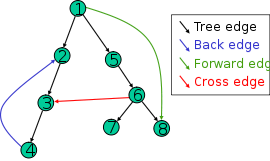
\includegraphics{edges.png}
\textbf{DAG:} Directed Acyclic Graph (tree is a DAG).\textbf{Partial order:} $a>b,b>c \rightarrow a>c$ but maybe a=b. \textbf{Total order:} Always $a>b$ or $a<b$.\\
\textbf{Topological Sort:} On DAG, no back edges. $\Theta(V+E)$. \textbf{Strongly Connectd Component } if we can reach u from v, for any u and v in a subset of G. $G^T$ has edges flipped (forward=backward).\\
\textbf{Compute SCC:} DFS(G), then $G^T$, then DFS($G^T$) (in order of deacreasing f[u], as computed by DFS(G)).\\
\textbf{d[u]:} start time.\textbf{f[u]:} finish time.\\
\textbf{MST: }Connect all edges. Cut respects A - no edge in A crosses it.\textbf{ Safe edge}: smallest weight edge between A and V-A.\\
\textbf{Kruskal:}\\
1. Starts	with	each	vertex	in	its	own	component (1 partition / vertex).	\\
2. Repeatedly	merges	two	components	into	one	by	choosing	a	
light	edge	that	connects	them	(i.e.,	a	light	edge	crossing	the	
cut	between	them).	\\
3. Scans	the	set	of	edges	in	monotonically	increasing	order	by	
weight.	\\
4. Uses	a	 disjoint-set	data	structure	 to	determine	whether	an	
edge	connects	vertices	in	different	components.\\
Union by rank + path compression : total runtime = O(E log V)\\
\textbf{Prim's Algorithm: }\\
1. Builds	 one	tree,	so	 A	 is	always	a	tree.	\\
2. Starts	from	an	arbitrary	 “root” r	 .	\\
3. At	each	step,	 adds	a	light	edge	 crossing	cut	 $(V_A, V	 - V_A)$ to A.
– Where	 $V_A$ = vertices	that	 A	 is	incident	on.\\
\textbf{Find a light edge (for Prim):}\\
1. Uses	a	 priority	queue	 Q	to	find	a		light	edge	quickly.\\	
2. Each	object	in	 Q	 is	a	vertex	in	V - VA.	\\
3. Key	of	 v is	minimum	weight	of	any	edge	 (u, v),	where	 u	 ∈ $V_A$.	\\
4. Then	the	vertex	returned	by	Extract-Min	is	 v such	that	there	
exists	 u	 ∈ V  and	 (u, v) is	light	edge	crossing	 $(V_A, V - V_A)$.	\\
5. Key	of	 v is	 ∞ if	 v is	not	adjacent	to	any	vertex	in	VA.\\
Prim - add lightest edges to neighbors until all reachable. Kruskal - connect partitions with safe edges until partition= whole graph.
\textbf{Shortest paths:} d[v]- \textbf{shortest path estimate.} (initially = $\infty$).$\pi[v]$ - predecessor of v (initially = NIL or if none).\\
\textbf{Relax an edge (if exists shorter path):}\\
if (d[v] $>$ d[u]+w(edge between u and v)) then d[v]=d[u]+w(edge between u and v), $\pi$[v]=u.\\
\textbf{Dijkstra: }\\
\begin{lstlisting}[frame=single]
DIJKSTRA( V, E,w, s)
INIT-SINGLE-SOURCE( V, s)
S = {}
Q = V
while Q non empty do
u = EXTRACT-MIN( Q)
S = S U {u}
for each vertex v ∈ Adj[ u] do
RELAX( u,v,w)
\end{lstlisting}
If we use binary heap, runtime = O(E log V)\\
\textbf{Gale-Shapley:} \\
\begin{lstlisting}[frame=single]
matching = empty
while there is a in A not yet matched do	
B =pref[a].removeFirst()	
if B not yet matched then
	 	 matching = matching U{(a,B)}	
else	
	 	 G = B current match 	
	 	 if B prefers a over G then
	 	 	 matching = matching -{(G,B)} U {(a,B)}
return matching
\end{lstlisting}
\textbf{Residual graph:}
\begin{lstlisting}[frame=single]
for each edge e=(u,v) in E
if f(e) < c(e)	
then {	
	 	 put a forward edge (u,v) in Residual graph
	 	 with residual capacity cf(e)=c(e)-f(e)	
}	
if f(e)>0	
then {	
	 	put a backward edge (v,u) in Residual graph
	 	with residual capacity cf(e)=f(e)	
}	
}	
\end{lstlisting}
\textbf{Augmenting path: }From source to sink via residual graph. Follow lines and add capacity as you go\\
Final solution: add G + residual graph paths . (take difference of edges flow if backwards + forward)\\
\textbf{Ford-Fulkerson:}\\
\begin{lstlisting}[frame=single]
f =0
Residual=G
while (there is a source to sink path in Residual){
f.augment(Path)
update Residual based on new f
}
\end{lstlisting}
\textbf{Flow through a cut: } $|f|=\sum f(e) from A to B - \sum f(e) from B to A$.\\
\textbf{Minimum cut: } \\
1. Run Ford-Fulkerson for max flow.\\
2. Run BFS /DFS from s.\\
3. All reachable vertices define the cut.
\end{document}